\documentclass[12pt, a4paper, twoside, openright]{book}

\usepackage{vuwthesis} % sets up some local things, mostly the front page

%\usepackage{palatino} % sets palatino as the default font

\usepackage{url} % for typesetting urls

\usepackage{docmute}



\usepackage{amssymb, amsmath}
\usepackage{tikz}

\newcommand{\vens}{\ensuremath{v_{\mathrm{ens}}}}



%\renewcommand{\baselinestretch}{1.00}


\begin{document}

\frontmatter
% Book style knows about front matter
% Report style doesn't so you need to set roman numbering etc yourself :-(

%%%%%%%%%%%%%%%%%%%%%%%%%%%%%%%%%%%%%%%%%%%%%%%%%%%%%%%

\title{The Title}
\author{The Author}

\subject{Computer Science}
\abstract{An abstract of fewer than 500 words must be included.}
% Books don't normally have abstracts, and this is a bit of a hack

% Uncomment the appropriate degree
\phd
%\mscthesisonly
%\mscwithhonours
%\mscbothparts
% \otherdegree{DEGREE OR DIPLOMA NAME}



%%%%%%%%%%%%%%%%%%%%%%%%%%%%%%%%%%%%%%%%%%%%%%%%%%%%%%%




\maketitle

\chapter*{Acknowledgments}\label{C:ack} 

Any acknowledgments should go in here, between the title page and the
table of contents.  The acknowledgments do not form a proper chapter,
and so don't get a number or appear in the table of contents.


\tableofcontents


%%%%%%%%%%%%%%%%%%%%%%%%%%%%%%%%%%%%%%%%%%%%%%%%%%%%%%%

% book style knows about mainmatter
% if you are using report style you will have to rest page numbering etc.
\mainmatter

%%%%%%%%%%%%%%%%%%%%%%%%%%%%%%%%%%%%%%%%%%%%%%%%%%%%%%%

% individual chapters included here

\chapter{Introduction}\label{C:intro}
The \textsf{vuwthesis} style attempts to do 2 things:
\begin{enumerate}
\item produce the correct front pages -- explained in Chapter \ref{C:ex};
\item meet the library requirement for the deposit of theses -- explained in Chapter \ref{C:lib}.
\end{enumerate}

We try to set the front pages up after the fashion of the example on p58
of the 2002 PhD handbook. (Available at
\url{http://www2.vuw.ac.nz/home/publications/phd_handbook.pdf}, March
2003).

I assume that you are using \textsf{report.sty} or, preferably,
\textsf{book.sty}. The book style has things like \verb+\frontmatter+
defined, which make life a little easier. 

Although the style alters the margins, and so on,  if you'd prefer to do
something else then feel free to set them all yourself. In this case you
will probably want to look at the \textsf{layout} package.
\chapter{The front pages}\label{C:ex}

You can declare:
\begin{itemize}
\item an author using  \verb+\author{}+ -- your full name;
\item a title using \verb+\title{}+-- ALL IN CAPITALS IN THE EXAMPLE, but we use \verb#\Large# and \verb#\bf#, so normal case will do;
\item a subject using \verb+\subject{}+-- probably Computer Science, but you can pick anything you like;
\item an abstract using \verb+\abstract{}+-- this should be fewer then 500 words for a PhD. The handbook states ``A length of about 300 words is recommended.'' The \textsf{book} style does not have an \verb+abstract+ environment defined, so this is a bit of a hack.
\end{itemize}

You can also specify what degree you are submitting the thesis for by using:
\begin{itemize}
\item  \verb+\phd+, which produces ``\ldots in fulfilment of \ldots Doctor of Philosophy''
\item  \verb+\mscthesisonly+, which produces ``\ldots in fulfilment of \ldots Master of Science''
\item  \verb+\mscwithhonours+, which produces ``\ldots in partial fulfilment of \ldots Master of Science with Honours''
\item  \verb+\mscbothparts+, which produces ``\ldots in partial fulfilment of \ldots Master of Science''
\item  \verb+\otherdegree{DEGREE OR DIPLOMA NAME}+, which produces ``\ldots in fulfilment of \ldots DEGREE OR DIPLOMA NAME''
\end{itemize}

\chapter{Library requirements}\label{C:lib}

This Chapter describes some things done to be in accordance with the `Library Requirements for the Deposit of Theses' booklet, which can be obtained from the VUW library.

\section{Font size}
\textit{12 point font is recommended.} 

Set this yourself with the \verb+12pt+ option to the document class.

\section{Single or double sided}
\textit{Typing on one side preferred, text on both sides acceptable for longer works.} 

Use the \verb+oneside+ or \verb+twoside+ option to the document class. The \textsf{book} class default is \verb+twoside+.


\section{Line spacing}
\textit{Lines should be double spaced, or at least 1.5 spaces apart.} 

1.5 spacing for 12 point is set using:
\begin{itemize}
\item \verb+\renewcommand{\baselinestretch}{1.24}+  
\end{itemize}

To set anything else use, e.g  \verb+\renewcommand{\baselinestretch}{1.0}+ in the preamble. See p 53 of \cite{GMS94} for more information.


\section{Margins}
\textit{Uniform margins of at least 4cm on binding side, other three sides to have at least 1.5 cm}

\LaTeX\ styles often leave a lot of white space, and \textsf{book} is no exception. We only have to worry about the binding side.

For \verb+twoside+ we use these settings:
\setlength{\textheight}{19.8cm}
\setlength{\oddsidemargin}{1.46cm}
\setlength{\evensidemargin}{0.83cm}

For \verb+oneside+, if we use:
\begin{verbatim}
\setlength{\textheight}{19.8cm}
\setlength{\oddsidemargin}{1.46cm}
\end{verbatim}

Then \textsf{book} gives a margin of 4cm on the binding side, and about 3.2cm elsewhere.

If you want to change these then use the \textsf{layout} package.

\section{Paper size}
\textit{High quality A4 paper, all pages of equal size}

Set this yourself with the \verb+a4paper+ option to the document class.
\chapter{Binding}\label{C:bin}

The Library states:
\begin{itemize}
\item Thesis must be fully bound and cased in cloth or buckram in optional colour. (I think they mean you can pick the colour!)
\item Author's surname and initials and (short) title lettered on spine. (The thesis's title, not the author's, presumably.)
\item Author's full name and full title lettered on front cover. (Again, the thesis's title, not the author's, presumably.)
\item Two copies of a PhD thesis and one copy of a Master's thesis must be deposited. A signed availability slip must accompany the thesis.
\item  The principal supervisor is responsible for the deposit.
\end{itemize}
\chapter{Lorem ipsum}
The following comes from \url{http://www.lipsum.com/} (March 2003).

\section{The standard Lorem Ipsum passage, used since the 1500s}
``Lorem ipsum dolor sit amet, consectetur adipisicing elit, sed do eiusmod tempor incididunt ut labore et dolore magna aliqua. Ut enim ad minim veniam, quis nostrud exercitation ullamco laboris nisi ut aliquip ex ea commodo consequat. Duis aute irure dolor in reprehenderit in voluptate velit esse cillum dolore eu fugiat nulla pariatur. Excepteur sint occaecat cupidatat non proident, sunt in culpa qui officia deserunt mollit anim id est laborum.'' 

\section{Section 1.10.32 of ``de Finibus Bonorum et Malorum'', written by Cicero in 45 BC} 
``Sed ut perspiciatis unde omnis iste natus error sit voluptatem accusantium doloremque laudantium, totam rem aperiam, eaque ipsa quae ab illo inventore veritatis et quasi architecto beatae vitae dicta sunt explicabo. Nemo enim ipsam voluptatem quia voluptas sit aspernatur aut odit aut fugit, sed quia consequuntur magni dolores eos qui ratione voluptatem sequi nesciunt. Neque porro quisquam est, qui dolorem ipsum quia dolor sit amet, consectetur, adipisci velit, sed quia non numquam eius modi tempora incidunt ut labore et dolore magnam aliquam quaerat voluptatem. Ut enim ad minima veniam, quis nostrum exercitationem ullam corporis suscipit laboriosam, nisi ut aliquid ex ea commodi consequatur? Quis autem vel eum iure reprehenderit qui in ea voluptate velit esse quam nihil molestiae consequatur, vel illum qui dolorem eum fugiat quo voluptas nulla pariatur?'' 

\section{1914 translation by H. Rackham} 
``But I must explain to you how all this mistaken idea of denouncing pleasure and praising pain was born and I will give you a complete account of the system, and expound the actual teachings of the great explorer of the truth, the master-builder of human happiness. No one rejects, dislikes, or avoids pleasure itself, because it is pleasure, but because those who do not know how to pursue pleasure rationally encounter consequences that are extremely painful. Nor again is there anyone who loves or pursues or desires to obtain pain of itself, because it is pain, but because occasionally circumstances occur in which toil and pain can procure him some great pleasure. To take a trivial example, which of us ever undertakes laborious physical exercise, except to obtain some advantage from it? But who has any right to find fault with a man who chooses to enjoy a pleasure that has no annoying consequences, or one who avoids a pain that produces no resultant pleasure?'' 

\section{Section 1.10.33 of ``de Finibus Bonorum et Malorum'', written by Cicero in 45 BC}
``At vero eos et accusamus et iusto odio dignissimos ducimus qui blanditiis praesentium voluptatum deleniti atque corrupti quos dolores et quas molestias excepturi sint occaecati cupiditate non provident, similique sunt in culpa qui officia deserunt mollitia animi, id est laborum et dolorum fuga. Et harum quidem rerum facilis est et expedita distinctio. Nam libero tempore, cum soluta nobis est eligendi optio cumque nihil impedit quo minus id quod maxime placeat facere possimus, omnis voluptas assumenda est, omnis dolor repellendus. Temporibus autem quibusdam et aut officiis debitis aut rerum necessitatibus saepe eveniet ut et voluptates repudiandae sint et molestiae non recusandae. Itaque earum rerum hic tenetur a sapiente delectus, ut aut reiciendis voluptatibus maiores alias consequatur aut perferendis doloribus asperiores repellat.'' 

\section{1914 translation by H. Rackham} 
``On the other hand, we denounce with righteous indignation and dislike men who are so beguiled and demoralized by the charms of pleasure of the moment, so blinded by desire, that they cannot foresee the pain and trouble that are bound to ensue; and equal blame belongs to those who fail in their duty through weakness of will, which is the same as saying through shrinking from toil and pain. These cases are perfectly simple and easy to distinguish. In a free hour, when our power of choice is untrammelled and when nothing prevents our being able to do what we like best, every pleasure is to be welcomed and every pain avoided. But in certain circumstances and owing to the claims of duty or the obligations of business it will frequently occur that pleasures have to be repudiated and annoyances accepted. The wise man therefore always holds in these matters to this principle of selection: he rejects pleasures to secure other greater pleasures, or else he endures pains to avoid worse pains.'' 

\documentclass[12pt, a4paper, twoside, openright]{book}

\usepackage{vuwthesis} % sets up some local things, mostly the front page

\setlength{\intextsep}{12pt} % set space above and below in-line float
\setlength{\abovecaptionskip}{0pt} % set space between figure and caption.

\usepackage{amssymb, amsmath}
\usepackage{tikz}

\usepackage{etoolbox}
\newtoggle{compilealone}
\toggletrue{compilealone}

\title{Replicating John Philip 1972}
\author{Nat Lund}

\begin{document}

\chapter{Replicating John Philip 1972}\label{C:jrphilip}

The first known expression for an effective slip length appeared in 1972, in a paper in ZAMP by John R. Philip entitled ``Flows Satisfying Mixed No-Slip and No-Shear Conditions" \cite{Philip1972}.

In the paper, John R. Philip says that the limit of
\begin{equation}
W_{3} = \Im \left[  
 \alpha^{-1} \cos^{-1} 
 \left\{ \frac{\cos(\alpha \Theta)}{\cos \alpha} \right\} - \Theta
   \right]
\end{equation}
as $y\rightarrow \infty$ is
\begin{equation}
W_{3} = \alpha^{-1} \ln \sec \alpha
\end{equation}

Let us prove this forthwith.
\vspace*{1em}

$\Theta = x + iy$ is a complex number, $\alpha$ is real.  Trig identities for \emph{complex} cosine and exponential:
\begin{gather}
%\arccos z = - i \ln (z + \sqrt{z^{2} - 1}) \\
\cos z = \frac{e^{iz}+e^{-iz}}{2} \\
e^{i \theta} = \cos \theta + i \sin \theta 
\end{gather}

\clearpage
\section{Expand cosine term, dump negligible parts}

In Euler's formula $e^{i\theta} = cis(\theta)$, if $\theta$ is \emph{real}, then $e^{i \theta}$ traces out the unit circle in $\mathbb{C}$, with $\theta$ being the angle.

\begin{figure}[h]
\centering
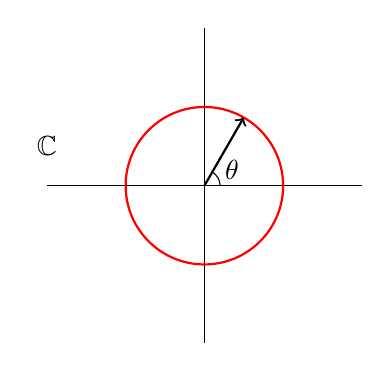
\begin{tikzpicture}
\draw (-2,0) -- ++ (4,0);
\draw (0,-2) -- ++(0,4);
\node at (-2,0.5) {$\mathbb{C}$};

\draw[thick, red] (0,0) circle (1cm);
\draw[thick,->] (0,0) -- ++(60:1);
\draw (0.2,0) arc  (0:60:2mm);
\node at (0.35,0.2) {$\theta$};

\end{tikzpicture}
\caption{Euler's formula $e^{i \theta}$ for real $\theta$ .}
\end{figure}


This gives insight into the $\cos z$ function.  If $z$ is real, then $\frac{1}{2} e^{iz}$ and $\frac{1}{2} e^{-iz}$ are two vectors of length $\frac{1}{2}$ that cycle in opposite directions, with $z$ being the angle. Then $\cos z$ is the sum of the two vectors, which always ends on the real line between -1 and 1, as shown in Figure (\ref{fig:cos}). 

\begin{figure}[h]
\centering
\begin{tikzpicture}
\draw (-4,0) -- ++ (8,0);
\draw (0,-2.5) -- ++(0,5);
\node at (-3,0.5) {$\mathbb{C}$};
\draw (4,0.1) -- ++(0,-0.2) node[below] {1};
\draw (-4,0.1) -- ++(0,-0.2) node[below] {-1};

\draw[thick, red, dashed] (0,0) circle (2cm);
\draw[thick, ->] (0,0) -- ++(45:2) -- ++(-45:2) node[below]{cos $z$};
\draw[thick, ->] (0,0) -- ++(45:2);
\node at (0.2,1)[right]{$\frac{1}{2} e^{iz}$};
\node at (2,1)[right]{$\frac{1}{2} e^{-iz}$};

\draw (0.3,0) arc  (0:45:3mm);
\node at (0.45,0.15) {$z$};

\draw[thick, dashed, ->] (0,0) -- ++(-45:2);
\draw (0.25,0) arc (0:-45:2.5mm);
\node at (0.5,-0.15) {$-z$};

\end{tikzpicture}
\caption{The complex cosine.} \label{fig:cos}
\end{figure}

With this insight, it is useful to rewrite $\cos z$ as:
\begin{equation}
\cos (x + iy) = \frac{ e^{i(x+iy)}+e^{-i(x+iy)} }{2} =
%\frac{ e^{ix - y} + e^{-ix + y} }{2} = 
e^{y} \frac{1}{2}e^{-ix} + e^{-y} \frac{1}{2} e^{ix}
\end{equation}

Then it is clear that $\cos (x + iy)$ is the sum of two rotating vectors in $\mathbb{C}$ with amplitudes $e^y$ and $e^{-y}$.  A consequence is that for large $y$, $e^y$ is \emph{very} large, while $e^{-y}$ is negligible, therefore $\cos (x + iy)$ is dominated by the vector $ e^{y} \frac{1}{2}e^{-ix} $.  See Figure (\ref{fig:coslargey}).

\begin{figure}[ht]
\centering
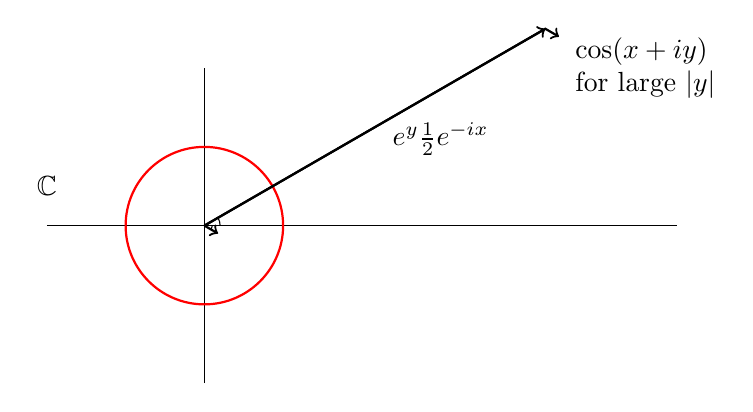
\begin{tikzpicture}
\draw (-2,0) -- ++ (8,0);
\draw (0,-2) -- ++(0,4);
\node at (-2,0.5) {$\mathbb{C}$};

\draw[thick, red] (0,0) circle (1cm);

\draw[thick,->] (0,0) -- ++(30:5) -- ++(-30:0.2);
\draw[thick,->] (0,0) -- ++(30:5);
\draw (0.2,0) arc  (0:30:2mm);
\draw[thick,->] (0,0) -- ++(-30:0.2);
\draw (0.1,0) arc (0:-30:1mm);

\node at (3,1.1) {$e^{y} \frac{1}{2}e^{-ix}$};
{
\renewcommand{\baselinestretch}{1.00}
\node at (5.6,2)[align=left] {$\cos (x+iy)$\\ for large $|y|$};
}
\end{tikzpicture}
\caption{Complex cosine at large $|y|$.} \label{fig:coslargey}
\end{figure}

\begin{equation}
\text{Therefore} \quad \cos (x + iy) \to  \frac{e^{y} e^{-ix}}{2}
\quad \text{as} \quad y \to \infty
\end{equation}

\begin{equation}
\cos z \to \frac{1}{2} e^{-iz} \quad \text{as} \quad y \to \infty
\end{equation}


\section{Inverse Cosine at Large $y$}

As $y \to \infty$:
\begin{equation}
w = \cos z \to \frac{1}{2} e^{-iz}
\end{equation}
Solve $w = \cos z$ for $z$ to get:
\begin{equation*}
\arccos w = z
\end{equation*}
Likewise solve $w = \frac{1}{2} e^{-iz}$ for $z$:
\begin{gather*}
w = \frac{1}{2} e^{-iz} \\
2 w = e^{-iz} \\
\ln (2w) = -iz \\
%\text{Multiply both sides by }i \\
i \ln (2w) = -i^2 z \\
%\text{Now, } -i^2 = 1, \text{  so} \\
i \ln (2w) = z
\end{gather*}
Equate the two expressions to obtain the inverse cosine in terms of a logarithm:
\begin{equation}
\arccos z = i \ln(2z)
\end{equation}

\section{Put into J.\ R.\ Philip's Expression}

\begin{equation}
W_{3} = \Im \left[  
 \alpha^{-1} \cos^{-1} 
 \left\{ \frac{\cos(\alpha \Theta)}{\cos \alpha} \right\} - \Theta
   \right]
\end{equation}

As $y \to \infty$, the cosine expression may be substituted:

\begin{equation}
W_{3} = \Im \left[  
 \alpha^{-1} \cos^{-1} 
 \left\{ \frac{\frac{1}{2} e^{-i \alpha \Theta}}{\cos \alpha} \right\} - \Theta
   \right]
\end{equation}

And the inverse cosine expression may also be substituted:

\begin{equation}
W_{3} = \Im \left[  
 i \alpha^{-1} \ln 
 \left\{ 2 \frac{\frac{1}{2} e^{-i \alpha \Theta}}{\cos \alpha} \right\} - \Theta
   \right]
\end{equation}

\begin{equation}
W_{3} = \Im \left[  
 i \alpha^{-1} \ln 
 \left\{ e^{-i \alpha \Theta} \frac{1 }{\cos \alpha} \right\} - \Theta
   \right]
\end{equation}

Recall that $\ln ab = \ln a + \ln b$.

\begin{equation}
W_{3} = \Im \left[  
 i \alpha^{-1} \ln 
 \left\{ e^{-i \alpha \Theta}  \right\}
+
i \alpha^{-1} \ln 
 \left\{ \frac{1 }{\cos \alpha} \right\} 
  - \Theta
   \right]
\end{equation}

Invoke definition of logarithm: $\ln e^z = z$.

\begin{equation}
W_{3} = \Im \left[  
 i \alpha^{-1} 
 \left\{ -i \alpha \Theta  \right\}
+
i \alpha^{-1} \ln 
 \left\{ \frac{1 }{\cos \alpha} \right\} 
  - \Theta
   \right]
\end{equation}

%\begin{equation}
%W_{3} = \Im \left[  
% -i^2 \alpha^{-1} \alpha \Theta
%+
%i \alpha^{-1} \ln 
% \left\{ \frac{1 }{\cos \alpha} \right\} 
%  - \Theta
%   \right]
%\end{equation}

\begin{equation}
W_{3} = \Im \left[  
\Theta
+
i \alpha^{-1} \ln 
 \left\{ \frac{1 }{\cos \alpha} \right\} 
  - \Theta
   \right]
\end{equation}

\begin{equation}
W_{3} = \Im \left[  
i \alpha^{-1} \ln 
 \left\{ \frac{1 }{\cos \alpha} \right\} 
   \right]
\end{equation}

%\begin{equation}
%W_{3} =
%\alpha^{-1} \ln 
% \left\{ \frac{1 }{\cos \alpha} \right\} 
%\end{equation}

\begin{equation}
W_{3} =
\alpha^{-1} \ln \sec \alpha
\end{equation}

We have demonstrated that which we set out to prove.
%As required.

\iftoggle{compilealone}
    {
    \bibliography{Lund_Thesis.bib}
    \bibliographystyle{plain}
    }

\end{document}





%The complex cosine term in J. R. Philip's expression is:
%\begin{equation}
%\left\{ \frac{\cos(\alpha \Theta)}{\cos \alpha} \right\} = 
%\left\{ \frac{\cos(\alpha(x + iy)}{\cos \alpha} \right\} =
%\left\{ \frac{\cos(\alpha x + i \alpha y)}{\cos \alpha} \right\}
%\end{equation}
%For any fixed real $\alpha$, as $y \to \infty$,
%\begin{equation}
%\left\{ \frac{\cos(\alpha x + i \alpha y)}{\cos \alpha} \right\} \to
%\left\{ \frac{ e^{\alpha y} e^{-i\alpha x} }{2 \cos \alpha} \right\}
%\end{equation}
%The magnitude of this complex number tends to infinity as $y \to \infty$.
%
%\end{document}


\chapter{Conclusions}\label{C:con}

If all the economists in the world were laid end-to-end they wouldn't
reach a conclusion, and neither shall I.




%%%%%%%%%%%%%%%%%%%%%%%%%%%%%%%%%%%%%%%%%%%%%%%%%%%%%%%

% and of course book style knows about backmatter
% \backmatter caused problems with appendices :-(
% and of course report style doesn't
%%%%%%%%%%%%%%%%%%%%%%%%%%%%%%%%%%%%%%%%%%%%%%%%%%%%%%%


%\bibliographystyle{ieeetr}
\bibliographystyle{acm}
\bibliography{myrefs}


\end{document}
